\documentclass[12pt]{article}

% UTF-8 encoding and fonts
\usepackage[utf8]{inputenc}
\usepackage[T1]{fontenc}
\usepackage{lmodern}

% Page setup
\usepackage[margin=1in]{geometry}
\usepackage{setspace}
\onehalfspacing

% Typography
\usepackage{microtype}

% Math and symbols
\usepackage{amsmath,amssymb}

% Graphics
\usepackage{graphicx}
\usepackage{float}
\usepackage{subcaption}

% Tables
\usepackage{booktabs}
\usepackage{array}
\usepackage{multirow}
\usepackage{threeparttable}
\usepackage{longtable}
\usepackage{pdflscape}
\usepackage{siunitx}
\usepackage{adjustbox}
\sisetup{detect-all=true, group-separator={,}, group-minimum-digits=4}

% Bibliography
\usepackage{natbib}
\bibliographystyle{aer}

% Hyperlinks
\usepackage{hyperref}
\hypersetup{
    colorlinks=true,
    linkcolor=blue,
    citecolor=blue,
    urlcolor=blue
}
\usepackage[nameinlink,noabbrev]{cleveref}

% Timing data
\IfFileExists{timing_data.tex}{\input{timing_data.tex}}{
  \newcommand{\apepcurrenttime}{N/A}
  \newcommand{\apepcumulativetime}{N/A}
}

% Captions
\usepackage{caption}
\captionsetup{font=small,labelfont=bf}

% Section formatting
\usepackage{titlesec}
\titleformat{\section}{\large\bfseries}{\thesection.}{0.5em}{}
\titleformat{\subsection}{\normalsize\bfseries}{\thesubsection}{0.5em}{}

% Custom commands
\newcommand{\E}{\mathbb{E}}
\newcommand{\Var}{\text{Var}}
\newcommand{\Cov}{\text{Cov}}
\newcommand{\ind}{\mathbb{I}}
\newcommand{\sym}[1]{\ifmmode^{#1}\else\(^{#1}\)\fi}

% modelsummary / tabularray support
\usepackage{tabularray}
\usepackage{codehigh}
\usepackage[normalem]{ulem}
\UseTblrLibrary{booktabs}
\UseTblrLibrary{siunitx}
\newcommand{\tinytableTabularrayUnderline}[1]{\underline{#1}}
\newcommand{\tinytableTabularrayStrikeout}[1]{\sout{#1}}
\NewTableCommand{\tinytableDefineColor}[3]{\definecolor{#1}{#2}{#3}}
\title{Council Tax Support Localisation and Low-Income Employment in England}
\author{APEP Autonomous Research\thanks{Autonomous Policy Evaluation Project. Correspondence: scl@econ.uzh.ch{} (cumulative: \apepcumulativetime{}).} \and @olafdrw}
\date{\today}

\begin{document}

\maketitle

\begin{abstract}
\noindent
In April 2013, the UK government replaced national Council Tax Benefit with locally administered Council Tax Support, allowing English local authorities to cut working-age support. I exploit cross-authority variation in the generosity of replacement schemes to estimate the effect of benefit reductions on claimant count rates using a panel of 276 local authorities over 2008--2023. A naive two-way fixed effects estimator yields a negative coefficient ($-$0.156 percentage points), but event-study diagnostics reveal significant pre-trends. After controlling for authority-specific linear trends, the sign reverses: CTS cuts \emph{increase} claimant rates by 0.152 percentage points ($p = 0.013$). However, restricting to the pre-COVID period renders both estimates insignificant. The sign reversal illustrates how standard TWFE can produce misleading conclusions when treatment groups differ in pre-existing trajectories.
\end{abstract}

\vspace{1em}
\noindent\textbf{JEL Codes:} H71, I38, J22 \\
\noindent\textbf{Keywords:} council tax support, welfare reform, localisation, employment, difference-in-differences

\newpage

\section{Introduction}

On 1 April 2013, the British government abolished Council Tax Benefit---a nationally uniform means-tested programme that had shielded 5.9 million low-income households from council tax liabilities---and replaced it with locally designed Council Tax Support (CTS) schemes administered by 326 English local authorities. The reform came with a 10 percent cut to the national grant, forcing authorities to choose: absorb the shortfall or pass it on to working-age claimants. Pensioner entitlements were protected by statute. The result was a dramatic divergence in the generosity of in-work support across English authorities, creating the largest subnational experiment in welfare localisation in recent British history \citep{ifs2013localising, nao2013localising}.

The policy interest in CTS localisation is straightforward. Cutting means-tested benefits for working-age households reduces marginal tax rates on earnings and should, according to standard labour supply theory, encourage employment \citep{moffitt2002welfare, saez2002optimal}. This logic---that less generous welfare means more work---has been central to UK welfare reform since the Welfare Reform Act 2012 and continues to animate debates over Universal Credit conditionality and benefit sanctions \citep{brewer2019did, beatty2014welfare}. Yet the same reductions push low-income households toward financial distress, debt, and housing instability, which may impair job search and employment retention \citep{jrf2015council, costa2019welfare}. Which effect dominates is an empirical question.

This paper estimates the causal effect of CTS cuts on local authority claimant count rates---the share of the working-age population receiving unemployment-related benefits---using a difference-in-differences design that exploits cross-authority variation in the generosity of replacement CTS schemes. I construct a treatment measure from DLUHC Council Taxbase data by computing working-age CTS per capita for each authority, residualised on the pre-reform claimant rate to separate policy generosity from underlying need \citep{dluhc2013taxbase}. The resulting continuous treatment variable captures how much each authority cut relative to what its demographic profile would predict.

My main finding is methodological as much as substantive: the two specifications tell opposite stories. A standard two-way fixed effects (TWFE) estimator with authority and month fixed effects yields a coefficient of $-$0.156 percentage points ($p < 0.001$), suggesting that CTS cuts \emph{reduced} claimant rates---the work incentive narrative. But event-study diagnostics reveal statistically significant pre-trends, with treatment and control authorities diverging well before April 2013. This pre-existing divergence invalidates the parallel trends assumption underlying the naive estimate.

Controlling for authority-specific linear time trends---a standard approach when pre-trends reflect differential trajectories rather than anticipation effects---flips the sign. The detrended estimate is $+$0.152 percentage points ($p = 0.013$): CTS cuts \emph{increased} claimant rates. A pre-reform placebo test yields a coefficient of $-$0.021 ($p = 0.47$), confirming that the detrended specification purges the confounding trends. The Rambachan--Roth sensitivity analysis under the HonestDiD framework shows that moderate violations of the parallel trends assumption are sufficient to change the sign of the naive estimate, further undermining the simple work incentive interpretation \citep{rambachan2023more}.

This paper contributes to three literatures. First, I add to the growing body of work on UK austerity and its local effects. \citet{fetzer2019austerity} showed that austerity-induced welfare losses predicted support for Brexit; I complement this by documenting direct labour market effects of the same suite of reforms. Where \citet{adam2019taxing} found null effects using cross-sectional variation, my panel event-study approach---tracking 276 authorities monthly over 16 years---provides both more statistical power and the diagnostics needed to separate causal effects from confounding trends.

Second, I speak to the broader debate on welfare conditionality and work incentives. The theoretical prediction that benefit cuts encourage employment assumes that the substitution effect dominates the income effect and that job search is unconstrained \citep{blundell2000employment, brewer2010labour}. My results suggest the opposite: for households near the bottom of the income distribution, losing council tax support may trigger a cascade of financial difficulties---arrears, enforcement action, debt---that undermines rather than improves labour market attachment. This echoes findings from the US context where aggressive benefit reductions have sometimes worsened outcomes for the most vulnerable \citep{blank2002evaluating, hoynes2016antipoverty}.

Third, I contribute methodologically by demonstrating the importance of pre-trend diagnostics in quasi-experimental policy evaluation. The sign reversal between naive and detrended estimates illustrates how standard TWFE can produce misleading conclusions when treatment and control groups were on different trajectories before the policy change---a concern formalised by \citet{goodmanbacon2021difference}, \citet{roth2023pretest}, and \citet{borusyak2024revisiting}. My analysis shows that this is not merely a theoretical possibility but a practical danger: the ``headline'' estimate supports the politically convenient narrative, while careful diagnostics reveal the opposite.

The remainder of the paper proceeds as follows. Section 2 describes the institutional background of CTS localisation. Section 3 develops a simple conceptual framework for understanding the competing channels. Section 4 presents the data. Section 5 details the empirical strategy. Section 6 reports results. Section 7 discusses mechanisms and implications. Section 8 concludes.



\section{Institutional Background}

\subsection{Council Tax Benefit: The National System (1993--2013)}

Council Tax Benefit (CTB) was introduced alongside Council Tax in 1993 as a nationally uniform means-tested benefit administered by local authorities on behalf of the Department for Work and Pensions. CTB reduced the council tax liability of low-income households, with maximum support equal to the full tax bill. The benefit was withdrawn at a taper rate of 20 percent of income above applicable amounts, creating high marginal effective tax rates for working claimants---a longstanding concern in UK tax-benefit design \citep{mirrlees2011tax, brewer2010labour}.

By 2012--13, CTB cost approximately \pounds 4.9 billion annually and supported 5.9 million households across England, Scotland, and Wales. Crucially, both pensioners and working-age households received identical treatment under the national rules. The DWP set all parameters: applicable amounts, tapers, non-dependant deductions, and earnings disregards. Local authorities had no discretion over generosity \citep{ifs2013localising}.

\subsection{The 2013 Localisation}

The Welfare Reform Act 2012 devolved responsibility for working-age council tax support to local authorities in England from April 2013. The reform had three key features.

\emph{Grant cut.} The national grant to fund CTS was reduced by approximately 10 percent---roughly \pounds 490 million---relative to the projected cost of maintaining CTB. Authorities had to design local schemes within this reduced budget \citep{nao2013localising}.

\emph{Pensioner protection.} Pensioner entitlements were ring-fenced at the pre-reform level by regulation. Any savings had to come exclusively from working-age claimants, concentrating the fiscal pressure on the most labour-market-relevant population.

\emph{Local discretion.} Each billing authority could design its own scheme, choosing whether and how to cut working-age support. Options included introducing minimum payments (requiring all working-age claimants to pay a proportion of their council tax), reducing the taper rate, capping support at a lower council tax band, or restricting second-adult rebates. Some authorities---particularly those with existing budgetary headroom or political preferences for protection---chose to fully fund the shortfall and maintain CTB-equivalent generosity.

The result was substantial cross-authority variation. According to the New Policy Institute, by 2014--15 minimum payments ranged from zero (authorities that maintained full passporting) to over 30 percent of the bill in the least generous schemes. The Joseph Rowntree Foundation documented that low-income households in the least generous authorities faced annual losses of \pounds 150--250, with knock-on effects for arrears and debt \citep{jrf2015council}.

\subsection{Why This Reform Provides Useful Variation}

Three features make CTS localisation attractive for causal identification. First, the timing is sharp: all authorities transitioned simultaneously on 1 April 2013, with no staggering. This eliminates concerns about dynamic treatment effects from heterogeneous adoption timing that complicate staggered difference-in-differences designs \citep{callaway2021difference, sun2021estimating}. Second, the treatment margin is well-defined: the only dimension of variation is the generosity of working-age CTS, since pensioner support was uniformly protected. Third, the reform was largely unanticipated in its specific design parameters---while localisation was announced in the 2010 Spending Review, individual authority schemes were not finalised until late 2012, limiting anticipation effects.

The main identification concern is selection: authorities that chose to cut CTS may differ systematically from those that maintained generosity. I address this by residualising the treatment measure on pre-reform claimant rates, by controlling for authority-specific linear trends, and by conducting extensive pre-trend diagnostics.

\subsection{The Broader Austerity Context}

CTS localisation did not occur in isolation. It was one element of the Welfare Reform Act 2012, which also introduced the overall benefit cap, the spare room subsidy (``bedroom tax''), and laid the groundwork for Universal Credit. The coincidence of multiple welfare reforms raises the question of whether CTS effects can be isolated from other policy changes. Two features of the research design address this concern. First, all of the other reforms applied nationally---they did not vary across local authorities in the same dimension as CTS generosity. The benefit cap, for instance, applied a uniform ceiling across England, and the bedroom tax applied uniform percentage reductions to housing benefit for under-occupying social tenants. These common shocks are absorbed by the month fixed effects in my specification. Second, the CTS treatment variable is constructed from authority-level data on actual CTS expenditure patterns, which reflect local discretionary choices rather than national policy parameters.

Nevertheless, interaction effects remain possible. Authorities that chose to cut CTS may also have been less effective at helping residents navigate other benefit changes, or may have had weaker local safety nets more broadly. The residualisation of the treatment variable on pre-reform claimant rates partially addresses this by removing the correlation between CTS generosity and baseline deprivation, but unmeasured dimensions of local capacity could still confound the estimate. I return to this limitation in the Discussion.

\subsection{Political Economy of Local Choices}

The variation in CTS generosity was not random. Authorities faced a classic fiscal choice: absorb the 10 percent grant cut from existing budgets (requiring cuts to other services or use of reserves) or pass some or all of the shortfall to working-age claimants. The political economy of this choice is relevant for interpreting the treatment variable.

Labour-controlled authorities were more likely to maintain full passporting (i.e., zero minimum payments for working-age claimants), while Conservative-controlled authorities were more likely to introduce minimum payments of 10--20 percent \citep{jrf2015council}. However, political control was not deterministic: some Conservative authorities in affluent areas could afford to absorb the cut, while some Labour authorities in deprived areas with tight budgets were forced to pass on costs. The correlation between political control and CTS generosity introduces a potential confounder if political party also affects employment outcomes through other channels. The authority-specific trends specification absorbs smooth political-economy effects to the extent that they evolve linearly over time.



\section{Conceptual Framework}

This section develops a simple framework for understanding the competing effects of CTS cuts on employment. The framework is deliberately minimalist: it identifies the key margins and generates testable predictions without imposing unnecessary structure.

\subsection{The Policy Margin}

Before April 2013, a low-income household in any English authority faced the same council tax support schedule. CTB reduced the household's council tax liability according to a national formula based on income, household composition, and local council tax rates. The effective marginal tax rate (EMTR) on earnings for a CTB recipient included a 20 percent taper: for every additional pound earned above the applicable amount, CTB was reduced by 20 pence.

After localisation, authorities could change three key parameters: (i) the minimum payment rate $m \in [0, 1]$, requiring all working-age claimants to pay at least fraction $m$ of their council tax bill; (ii) the taper rate $\tau$ at which CTS is withdrawn as income rises; and (iii) eligibility thresholds and earnings disregards. In practice, the most common change was the introduction of minimum payments, with $m$ typically between 0.08 and 0.30 across cut authorities.

\subsection{Work Incentive Channel}

Standard labour supply theory predicts that CTS cuts should increase employment through the substitution effect. Consider a household at the extensive margin (deciding whether to work at all). Under the national CTB scheme, the household paid zero council tax. Under a local CTS scheme with minimum payment $m$, the household now owes $m \times \text{CT}$ regardless of employment status. This creates a fixed cost of non-employment that did not exist before, which in principle should encourage work.

At the intensive margin, the effect depends on how CTS cuts change the EMTR schedule. If the taper rate $\tau$ is reduced, the EMTR falls and the substitution effect encourages more hours. If instead the authority simply imposes a minimum payment without changing the taper, the EMTR is unchanged and the intensive-margin substitution effect is zero. In practice, most authorities introduced minimum payments rather than taper changes, implying that the intensive-margin substitution effect was likely small \citep{adam2019taxing}.

Formally, let $h^*$ denote the household's optimal labour supply. The work incentive prediction is:
\begin{equation}
\frac{\partial h^*}{\partial m} > 0 \quad \text{(substitution effect)}
\end{equation}
because increasing the minimum payment raises the cost of non-employment relative to employment.

\subsection{Financial Distress Channel}

The competing prediction arises from the income effect and the constraints facing households at the bottom of the income distribution. CTS cuts reduce disposable income for non-working and low-earning households. For a household that was previously fully passported (paying zero council tax), a minimum payment of 20 percent on a Band B property in a northern authority represents approximately \pounds 3--4 per week---a non-trivial amount for a household living on \pounds 73.10 per week in Jobseeker's Allowance.

Three mechanisms connect this income loss to worse employment outcomes:

\emph{Debt and enforcement cascading.} Council tax is a priority debt---non-payment triggers a summons (\pounds 80--120 costs), liability order, and potentially bailiff enforcement. For households already managing multiple debts (rent, utilities, consumer credit), an unexpected council tax liability can trigger a cascade that consumes time and cognitive resources that would otherwise support job search \citep{chetty2013using}.

\emph{Housing instability.} Council tax arrears can lead to attachment of earnings orders and, in extreme cases, committal proceedings. The threat of enforcement action creates anxiety and instability that is antithetical to sustained job search and employment retention.

\emph{Administrative burden.} The transition from a national to a local scheme created confusion. Many households did not understand that they now owed council tax, did not know the amount, or did not receive bills on time. The administrative shock of the transition itself---separate from the financial impact---may have disrupted employment for affected households.

The financial distress prediction is:
\begin{equation}
\frac{\partial h^*}{\partial m} < 0 \quad \text{(income + distress effects)}
\end{equation}

\subsection{Testable Predictions}

The sign of the reduced-form effect of CTS cuts on employment is therefore ambiguous ex ante. However, the framework generates several auxiliary predictions:

\begin{enumerate}
\item \textbf{Dose-response:} If CTS cuts have a causal effect (in either direction), the effect should be stronger where cuts are deeper. Authorities in the bottom tercile of CTS generosity should show larger effects than those in the middle tercile.

\item \textbf{Pre-reform null:} Since the policy variation did not exist before April 2013, any specification that examines a placebo reform date in the pre-period should yield a null effect.

\item \textbf{Dynamic pattern:} Work incentive effects should appear relatively quickly (within 1--2 quarters as households adjust labour supply). Financial distress effects may appear with a lag (as arrears accumulate and enforcement escalates) or immediately (if the announcement itself disrupts behaviour).
\end{enumerate}



\section{Data}

\subsection{Claimant Count}

The primary outcome is the monthly claimant count rate: the number of people claiming unemployment-related benefits as a share of the working-age (16--64) population. I obtain claimant counts from the NOMIS database maintained by the Office for National Statistics, covering all 326 English local authority districts from January 2008 to December 2023---192 monthly observations per authority \citep{ons2023nomis}.

The claimant count captures individuals receiving Jobseeker's Allowance (until 2018) and subsequently those in the ``searching for work'' conditionality group under Universal Credit. While not a perfect measure of unemployment, it is the most granular monthly indicator of labour market distress available at the local authority level and is widely used in UK labour economics \citep{gregg2005proportion, manning2014coase}.

\subsection{Treatment Variable}

I construct the treatment variable from the 2013 Council Taxbase dataset published by the Department for Levelling Up, Housing and Communities (DLUHC). This records the number of Band D equivalent council tax support cases and their aggregate value, separately for pensioners and working-age claimants, for each English billing authority \citep{dluhc2013taxbase}.

The key measure is working-age CTS per working-age person (\pounds per year), computed by dividing total working-age CTS expenditure by ONS mid-year population estimates for 2012. To separate policy generosity from underlying need, I residualise this measure on the pre-reform mean claimant rate (2010--2012). The residual captures how generous each authority is \emph{relative to what its claimant profile would predict}: a positive residual indicates an authority providing more CTS than expected given its level of labour market disadvantage; a negative residual indicates one that cut more deeply.

The binary treatment variable classifies authorities below the median residual as ``cut'' ($N = 138$) and those above as ``protected'' ($N = 138$). I also construct a continuous treatment (standardised residual) and tercile groups for dose-response analysis.

\subsection{Population Data}

Working-age population estimates (ages 16--64) come from ONS mid-year population estimates accessed via NOMIS, covering 2008--2023 at the local authority level. These are used both to construct the claimant rate denominator and to normalise the treatment variable.

\subsection{Sample Construction}

The final analysis panel consists of 52,992 authority-month observations covering 276 English local authorities over 192 months (January 2008 to December 2023). The sample drops from 326 to 276 authorities after requiring successful linkage between NOMIS geography codes (ONS GSS codes) and DLUHC billing authority codes, non-missing population data, and non-missing treatment classification. I match NOMIS and DLUHC codes by authority name, using fuzzy matching (Levenshtein distance $\leq 5$) for cases where naming conventions differ across administrative datasets. The matched sample covers 85 percent of English authorities. The 50 unmatched authorities are predominantly small district councils affected by boundary changes or naming differences between ONS and DLUHC classification systems. A comparison of pre-reform claimant rates between matched and unmatched authorities (where both are observable in NOMIS) shows no systematic differences in baseline labour market conditions, though the unmatched set is somewhat skewed toward smaller, rural authorities.

\subsection{Summary Statistics}

\Cref{tab:summary} presents summary statistics by treatment group. Cut and protected authorities are similar in pre-reform claimant rates (1.99 versus 2.02 percent) and working-age population (181,000 versus 171,000). Post-reform, the gap widens: protected authorities retain higher claimant rates (1.83 versus 1.65 percent), consistent with the raw correlation between CTS generosity and claimant levels---though this comparison confounds treatment effects with pre-existing trends, as the event-study analysis will show.

\begin{table}[H]
\centering
\caption{Summary Statistics by Treatment Group}
\label{tab:summary}
\begin{threeparttable}
\begin{tabular}{lcc}
\toprule
& Cut LAs & Protected LAs \\
\midrule
N (local authorities) & 138 & 138 \\
Mean working-age population & 180,886 & 171,176 \\
Mean CTS per capita (\pounds) & 29.00 & 43.30 \\
\addlinespace
\emph{Pre-reform (Jan 2008--Mar 2013)} & & \\
\quad Mean claimant rate (\%) & 1.99 & 2.02 \\
\quad SD claimant rate (\%) & 0.97 & 0.94 \\
\addlinespace
\emph{Post-reform (Apr 2013--Dec 2023)} & & \\
\quad Mean claimant rate (\%) & 1.65 & 1.83 \\
\quad SD claimant rate (\%) & 1.00 & 1.11 \\
\bottomrule
\end{tabular}
\begin{tablenotes}[flushleft]
\small
\item \emph{Notes:} $N = 52{,}992$ authority-month observations across 276 English local authorities, January 2008 to December 2023. Treatment groups are defined by the \emph{residual} CTS per capita (after partialling out pre-reform claimant rates): ``Cut LAs'' have below-median residual generosity. The raw CTS per capita means reported here differ from the overall sample median (\pounds 33.18) because the binary split is on the residual, not the raw measure. Claimant rate is the monthly claimant count divided by working-age population.
\end{tablenotes}
\end{threeparttable}
\end{table}



\section{Empirical Strategy}

\subsection{Identification}

I estimate the effect of CTS cuts on claimant rates using a difference-in-differences design that compares authorities with less generous CTS schemes (``cut'') to those that maintained generosity (``protected''), before and after the April 2013 reform.

The identifying assumption is parallel trends: absent the differential CTS cuts, claimant rates in cut and protected authorities would have evolved along parallel paths. Because the reform affected all authorities simultaneously, this is a canonical two-group, two-period DiD design extended to a monthly panel---avoiding the heterogeneous treatment timing problems formalised by \citet{goodmanbacon2021difference} and \citet{dechaisemartin2020two}.

\subsection{Estimation}

The primary specification is:
\begin{equation}
\label{eq:main}
Y_{at} = \alpha_a + \gamma_t + \beta \cdot \text{Cut}_a \times \text{Post}_t + \varepsilon_{at}
\end{equation}
where $Y_{at}$ is the claimant rate in authority $a$ in month $t$, $\alpha_a$ are authority fixed effects, $\gamma_t$ are month fixed effects, $\text{Cut}_a$ is the binary treatment indicator, and $\text{Post}_t = \ind[t \geq \text{April 2013}]$. The coefficient $\beta$ captures the average effect of CTS cuts on claimant rates. Standard errors are clustered at the authority level to account for serial correlation within authorities \citep{angrist1999empirical}.

I supplement the binary specification with a continuous treatment version:
\begin{equation}
Y_{at} = \alpha_a + \gamma_t + \delta \cdot \text{CTS Intensity}_a \times \text{Post}_t + \varepsilon_{at}
\end{equation}
where $\text{CTS Intensity}_a$ is the standardised residual CTS per capita.

\subsection{Event Study}

To assess pre-trends and trace the dynamic treatment effect, I estimate an event-study specification with quarterly leads and lags:
\begin{equation}
\label{eq:eventstudy}
Y_{at} = \alpha_a + \gamma_t + \sum_{q \neq -1} \mu_q \cdot \text{Cut}_a \times \ind[Q_{at} = q] + \varepsilon_{at}
\end{equation}
where $Q_{at}$ indexes quarters relative to the reform (April 2013 $= 0$), with $q = -1$ as the reference period. The coefficients $\{\mu_q\}$ trace the treatment-control gap over time. Under parallel trends, pre-reform coefficients should be jointly zero. Significant pre-reform coefficients indicate differential trends that confound the main estimate \citep{roth2023pretest}.

\subsection{Authority-Specific Trends}

When event-study diagnostics reveal pre-trends, I augment the specification with authority-specific linear time trends:
\begin{equation}
\label{eq:trends}
Y_{at} = \alpha_a + \gamma_t + \lambda_a \cdot t + \beta^{\text{trend}} \cdot \text{Cut}_a \times \text{Post}_t + \varepsilon_{at}
\end{equation}
The authority-specific trend $\lambda_a \cdot t$ absorbs smooth differential trajectories between authorities, isolating the discrete break at April 2013. This approach is appropriate when pre-trends reflect gradually diverging fundamentals (e.g., differing local economic trajectories) rather than anticipation of the reform itself \citep{meyer1995natural}. I estimate this allowing for authority-specific slopes within the fixed effects framework.

\subsection{Threats to Validity}

\emph{Selection into treatment.} Authorities that cut CTS may differ from those that maintained generosity in ways that affect labour market outcomes. The treatment measure is residualised on pre-reform claimant rates to remove the most obvious confounder (baseline labour market conditions), and summary statistics confirm balance on observables. Authority and month fixed effects absorb all time-invariant authority characteristics and common shocks.

\emph{Pre-existing trends.} The main threat, confirmed by event-study diagnostics. I address this with authority-specific linear trends and assess sensitivity using the \citet{rambachan2023more} framework, which provides identified sets for the treatment effect under specified bounds on the degree of non-parallel trends.

\emph{Spillovers.} If workers relocate across authority boundaries in response to CTS changes, my estimates capture net effects (direct plus displacement). \citet{manning2014coase} find that UK local labour markets are relatively self-contained, suggesting limited cross-authority spillovers at the monthly frequency.

\emph{Compositional changes.} The claimant count definition changed with the rollout of Universal Credit (2013--2018). Since UC rollout varied across authorities, this is a potential confounder. Month fixed effects absorb national-level changes in the claimant count definition, and authority-specific trends absorb differential UC rollout timing to the extent that it follows a smooth trajectory.

\emph{COVID-19.} The 2020--2021 pandemic caused a massive, non-linear spike in claimant rates across all authorities. Month fixed effects absorb the common component of this shock, but differential COVID impacts across cut and protected authorities could confound the estimate. This is a first-order concern: restricting the sample to the pre-2020 period (January 2008 to December 2019; $N = 39{,}744$) yields a naive TWFE estimate of $-$0.041 ($p = 0.26$) and a trend-adjusted estimate of $+$0.032 ($p = 0.40$)---both statistically insignificant. The sign pattern is preserved (negative naive, positive detrended), but the magnitudes are smaller and neither estimate is distinguishable from zero. This implies that much of the statistical power in the full-sample estimates comes from differential claimant rate dynamics during and after the pandemic. I report the full-sample results as the primary specification because they exploit the full available variation, but the pre-2020 subsample analysis suggests that the CTS effect on pre-pandemic labour markets was modest at best.


\section{Results}

\subsection{Main Results}

\Cref{tab:main} presents the main results across five specifications. Column (1) reports the naive TWFE estimate from Equation~\ref{eq:main}: CTS cuts are associated with a reduction in claimant rates of 0.156 percentage points ($p < 0.001$). Taken at face value, this implies that reducing working-age council tax support improved employment outcomes---supporting the work incentive channel.

Column (2) uses the continuous treatment measure (standardised residual CTS per capita). The coefficient is positive ($+$0.077, $p = 0.012$), suggesting that more generous authorities had higher claimant rates---but this conflates treatment effects with pre-existing differences.

Column (3) introduces authority-specific linear time trends. The coefficient reverses sign to $+$0.152 percentage points ($p = 0.013$): after controlling for differential pre-trends, CTS cuts \emph{increase} claimant rates. This is the central finding. The sign flip reveals that the naive negative estimate was driven by cut authorities already being on a steeper downward claimant trajectory before the reform, not by a causal effect of the policy.

Columns (4) and (5) use log claimant rate as the dependent variable. The pattern is similar: the naive estimate is negative ($-$0.086), while the trend-adjusted estimate is positive, though imprecisely estimated in the log specification.

\begin{table}[H]
\centering
\caption{Effect of CTS Cuts on Claimant Rates}
\label{tab:main}
\begin{adjustbox}{max width=\textwidth}
\begin{threeparttable}
\begin{tabular}{lccccc}
\toprule
& (1) & (2) & (3) & (4) & (5) \\
& TWFE & Continuous & LA Trends & Log & Log + Trends \\
\midrule
Cut $\times$ Post & $-$0.156*** & & 0.152** & $-$0.086*** & 0.052 \\
& (0.029) & & (0.061) & (0.015) & (0.034) \\
CTS Intensity $\times$ Post & & 0.077** & & & \\
& & (0.030) & & & \\
\addlinespace
LA fixed effects & Yes & Yes & Yes & Yes & Yes \\
Month fixed effects & Yes & Yes & Yes & Yes & Yes \\
LA-specific trends & No & No & Yes & No & Yes \\
\addlinespace
Observations & 52,992 & 52,992 & 52,992 & 52,992 & 52,992 \\
\bottomrule
\end{tabular}
\begin{tablenotes}[flushleft]
\footnotesize
\item \emph{Notes:} Clustered SEs in parentheses. * $p<0.10$, ** $p<0.05$, *** $p<0.01$. Dependent variable: claimant rate (\%) in (1)--(3); log(claimant rate $+$ 0.01) in (4)--(5). ``Cut'' = below-median residual CTS per capita. ``CTS Intensity'' = standardised residual. (3) and (5) include LA-specific linear trends. $N = 276$ LAs, Jan 2008--Dec 2023.
\end{tablenotes}
\end{threeparttable}
\end{adjustbox}
\end{table}


\subsection{Event Study}

\Cref{fig:eventstudy} plots the event-study coefficients from Equation~\ref{eq:eventstudy}. The raw TWFE specification (red) shows a clear pattern of pre-existing divergence: coefficients at $q = -2$ ($-$0.036, $p < 0.001$), $q = -4$ ($-$0.034, $p = 0.014$), $q = -6$ ($-$0.066, $p < 0.001$), and $q = -7$ ($-$0.056, $p = 0.018$) are all significantly negative. Cut authorities were already experiencing declining claimant rates relative to protected authorities for at least two years before the reform.

The detrended specification (blue) removes this pre-existing divergence. Pre-reform coefficients cluster tightly around zero, while post-reform coefficients are small and statistically insignificant---consistent with a modest positive effect that does not grow dramatically over time. The contrast between the two event studies is the single most important piece of evidence in this paper: it demonstrates that the naive estimate is confounded and that careful pre-trend analysis is essential.

\begin{figure}[H]
\centering

\includegraphics[width=0.95\textwidth]{figures/fig2_event_study.png}
\caption{Event Study: Effect of CTS Cuts on Claimant Rates}
\label{fig:eventstudy}
\floatfoot{\emph{Notes:} Quarterly coefficients from Equation~\ref{eq:eventstudy}, with $q = -1$ as reference. The red series shows the raw TWFE event study; the blue series controls for authority-specific linear trends. Shaded areas are 95 percent confidence intervals based on standard errors clustered at the authority level. The dashed vertical line marks the reform date (April 2013). $N = 52{,}992$ authority-month observations across 276 local authorities.}
\end{figure}


\subsection{Dose-Response}

If CTS cuts causally affect claimant rates, the effect should be stronger where cuts were deeper. \Cref{tab:dose} presents results by tercile of CTS generosity, with the most protected authorities as the reference group. In the raw TWFE specification, the most-cut tercile shows a coefficient of $-$0.234 percentage points and the moderately-cut tercile shows $-$0.127 percentage points---a monotonic dose-response pattern. However, this gradient also reflects the pre-existing trends, since authorities with deeper cuts were on steeper downward trajectories. In the trend-adjusted specification, both coefficients turn positive and significant, but the dose-response gradient does not follow the expected monotonic pattern---the moderate-cut tercile shows a larger positive coefficient than the most-cut tercile. This reversal is consistent with the pre-existing trends confounding the naive estimates differently across terciles, rather than reflecting a true causal gradient.

\begin{table}[H]
\centering
\caption{Dose-Response: Effect by Tercile of CTS Cut Intensity}
\label{tab:dose}
\begin{threeparttable}
\begin{tabular}{lcc}
\toprule
& (1) Raw TWFE & (2) LA Trends \\
\midrule
Most Cut $\times$ Post & $-$0.234*** & 0.182** \\
& (0.042) & (0.078) \\
Moderate Cut $\times$ Post & $-$0.127*** & 0.342*** \\
& (0.036) & (0.074) \\
\addlinespace
Reference group & \multicolumn{2}{c}{Most Protected (T3)} \\
LA-specific trends & No & Yes \\
Observations & 52,992 & 52,992 \\
\bottomrule
\end{tabular}
\begin{tablenotes}[flushleft]
\small
\item \emph{Notes:} Standard errors clustered at the local authority level in parentheses. * $p<0.10$, ** $p<0.05$, *** $p<0.01$. Terciles are based on residual CTS per working-age person (residualised on pre-reform claimant rate). ``Most Cut'' = bottom tercile (lowest CTS generosity); ``Most Protected'' = top tercile (reference). All specifications include authority and month fixed effects.
\end{tablenotes}
\end{threeparttable}
\end{table}


\subsection{Robustness}

\Cref{tab:robust} and \Cref{fig:robust} present robustness checks. The results consistently tell the same story: the naive estimate is negative but driven by pre-trends, while specifications that address pre-trends yield null or positive effects.

\emph{Donut specification.} Excluding the 13 months closest to the reform (months $-6$ through $+6$ relative to April 2013) yields a coefficient of $-$0.164 ($p < 0.001$), slightly larger in magnitude than the baseline. This confirms that the negative estimate is not driven by transition-period dynamics. However, this specification does not address pre-existing trends and is therefore similarly confounded.

\emph{Pre-reform placebo.} Restricting the sample to the pre-reform period (2008--2013) and defining a placebo ``post'' period at October 2010 yields a coefficient of $-$0.021 ($p = 0.47$). The precise null confirms that the treatment-control gap does not exhibit discrete jumps at arbitrary dates---the pre-trends are smooth, which is exactly the pattern that authority-specific linear trends are designed to absorb.

\emph{Leave-one-out.} Dropping each of the ten largest authorities in turn produces estimates ranging from $-$0.168 to $-$0.161 in the naive specification, confirming that no single large authority drives the baseline result.

\emph{HonestDiD sensitivity.} The \citet{rambachan2023more} framework allows me to assess how robust the main estimate is to violations of parallel trends. The analysis shows that even modest departures from parallel trends (linear trend differences of $M = 0.01$ per quarter) are sufficient to shift the identified set to include zero, and larger departures ($M \geq 0.03$) flip the sign. This is consistent with the authority-specific trend result: the data cannot distinguish between ``CTS cuts reduced claimant rates'' and ``cut authorities were already improving faster'' without imposing functional form assumptions on the trend.

\emph{Quadratic trends.} Replacing linear authority-specific trends with quadratic trends yields a coefficient of $+$0.056 ($p = 0.31$), intermediate between the linear-trend and naive estimates but statistically insignificant. The sensitivity of the estimate to the functional form of the trend confirms that the sign and significance of the treatment effect depend on assumptions about the trend structure.

\emph{Pre-2020 subsample.} Restricting the sample to the pre-COVID period (January 2008 to December 2019; $N = 39{,}744$) yields a naive estimate of $-$0.041 ($p = 0.26$) and a trend-adjusted estimate of $+$0.032 ($p = 0.40$). Neither is statistically significant, although the sign pattern is preserved. This suggests that the COVID-era claimant spike differentially affected cut and protected authorities, amplifying the treatment-control gap in the full sample.

\begin{table}[H]
\centering
\caption{Robustness Checks}
\label{tab:robust}
\begin{adjustbox}{max width=\textwidth}
\begin{threeparttable}
\begin{tabular}{lcccccc}
\toprule
& (1) Main & (2) LA Trends & (3) Donut & (4) Placebo & (5) Quadratic & (6) Pre-2020 \\
\midrule
Cut $\times$ Post & $-$0.156*** & 0.152** & $-$0.164*** & $-$0.021 & 0.056 & $-$0.041 \\
& (0.029) & (0.061) & (0.031) & (0.029) & (0.055) & (0.036) \\
\addlinespace
LA-specific trends & Linear & Linear & No & No & Quadratic & No \\
Observations & 52,992 & 52,992 & 49,404 & 17,388 & 52,992 & 39,744 \\
\bottomrule
\end{tabular}
\begin{tablenotes}[flushleft]
\small
\item \emph{Notes:} Clustered SEs in parentheses. * $p<0.10$, ** $p<0.05$, *** $p<0.01$. All include LA and month FE. (2) LA-specific linear trends. (3) excludes months $-6$ to $+6$ around April 2013. (4) pre-reform only with placebo at Oct 2010. (5) LA-specific quadratic trends. (6) pre-COVID (Jan 2008--Dec 2019).
\end{tablenotes}
\end{threeparttable}
\end{adjustbox}
\end{table}

\begin{figure}[H]
\centering

\includegraphics[width=0.85\textwidth]{figures/fig5_robustness.png}
\caption{Robustness of Main Estimate Across Specifications}
\label{fig:robust}
\floatfoot{\emph{Notes:} Point estimates with 95 percent confidence intervals from alternative specifications. The five specifications are: Main TWFE (binary treatment), LA-specific linear trends, working-age CTS share (continuous, standardised), donut (excluding $\pm$6 months), and pre-reform placebo. All specifications include authority and month fixed effects with standard errors clustered at the authority level.}
\end{figure}


\subsection{Trends and Raw Data}

\Cref{fig:trends} plots mean claimant rates for cut and protected authorities over the full sample period. Both groups follow strikingly similar paths through the Great Recession (2008--2009), the recovery period (2010--2012), and the post-reform decline (2013--2017). The gap between groups is small and fluctuates. Visually, there is no obvious divergence at the reform date---consistent with either a null effect or an effect masked by pre-existing trends.

\begin{figure}[H]
\centering

\includegraphics[width=0.9\textwidth]{figures/fig1_trends.png}
\caption{Claimant Rate Trends by CTS Generosity}
\label{fig:trends}
\floatfoot{\emph{Notes:} Monthly mean claimant rates for cut and protected local authorities. ``Cut LAs'' are those with below-median residual CTS per capita; ``Protected LAs'' are above-median. The dashed vertical line marks April 2013 (CTS localisation). $N = 276$ local authorities.}
\end{figure}

\Cref{fig:dose_trends} disaggregates by tercile, showing that the most-cut authorities (T1) had consistently lower claimant rates than the most-protected authorities (T3) throughout the sample---a level difference that predates the reform and reflects the correlation between CTS generosity and underlying labour market conditions. The reform date does not produce a visible change in the gap between terciles.

\begin{figure}[H]
\centering
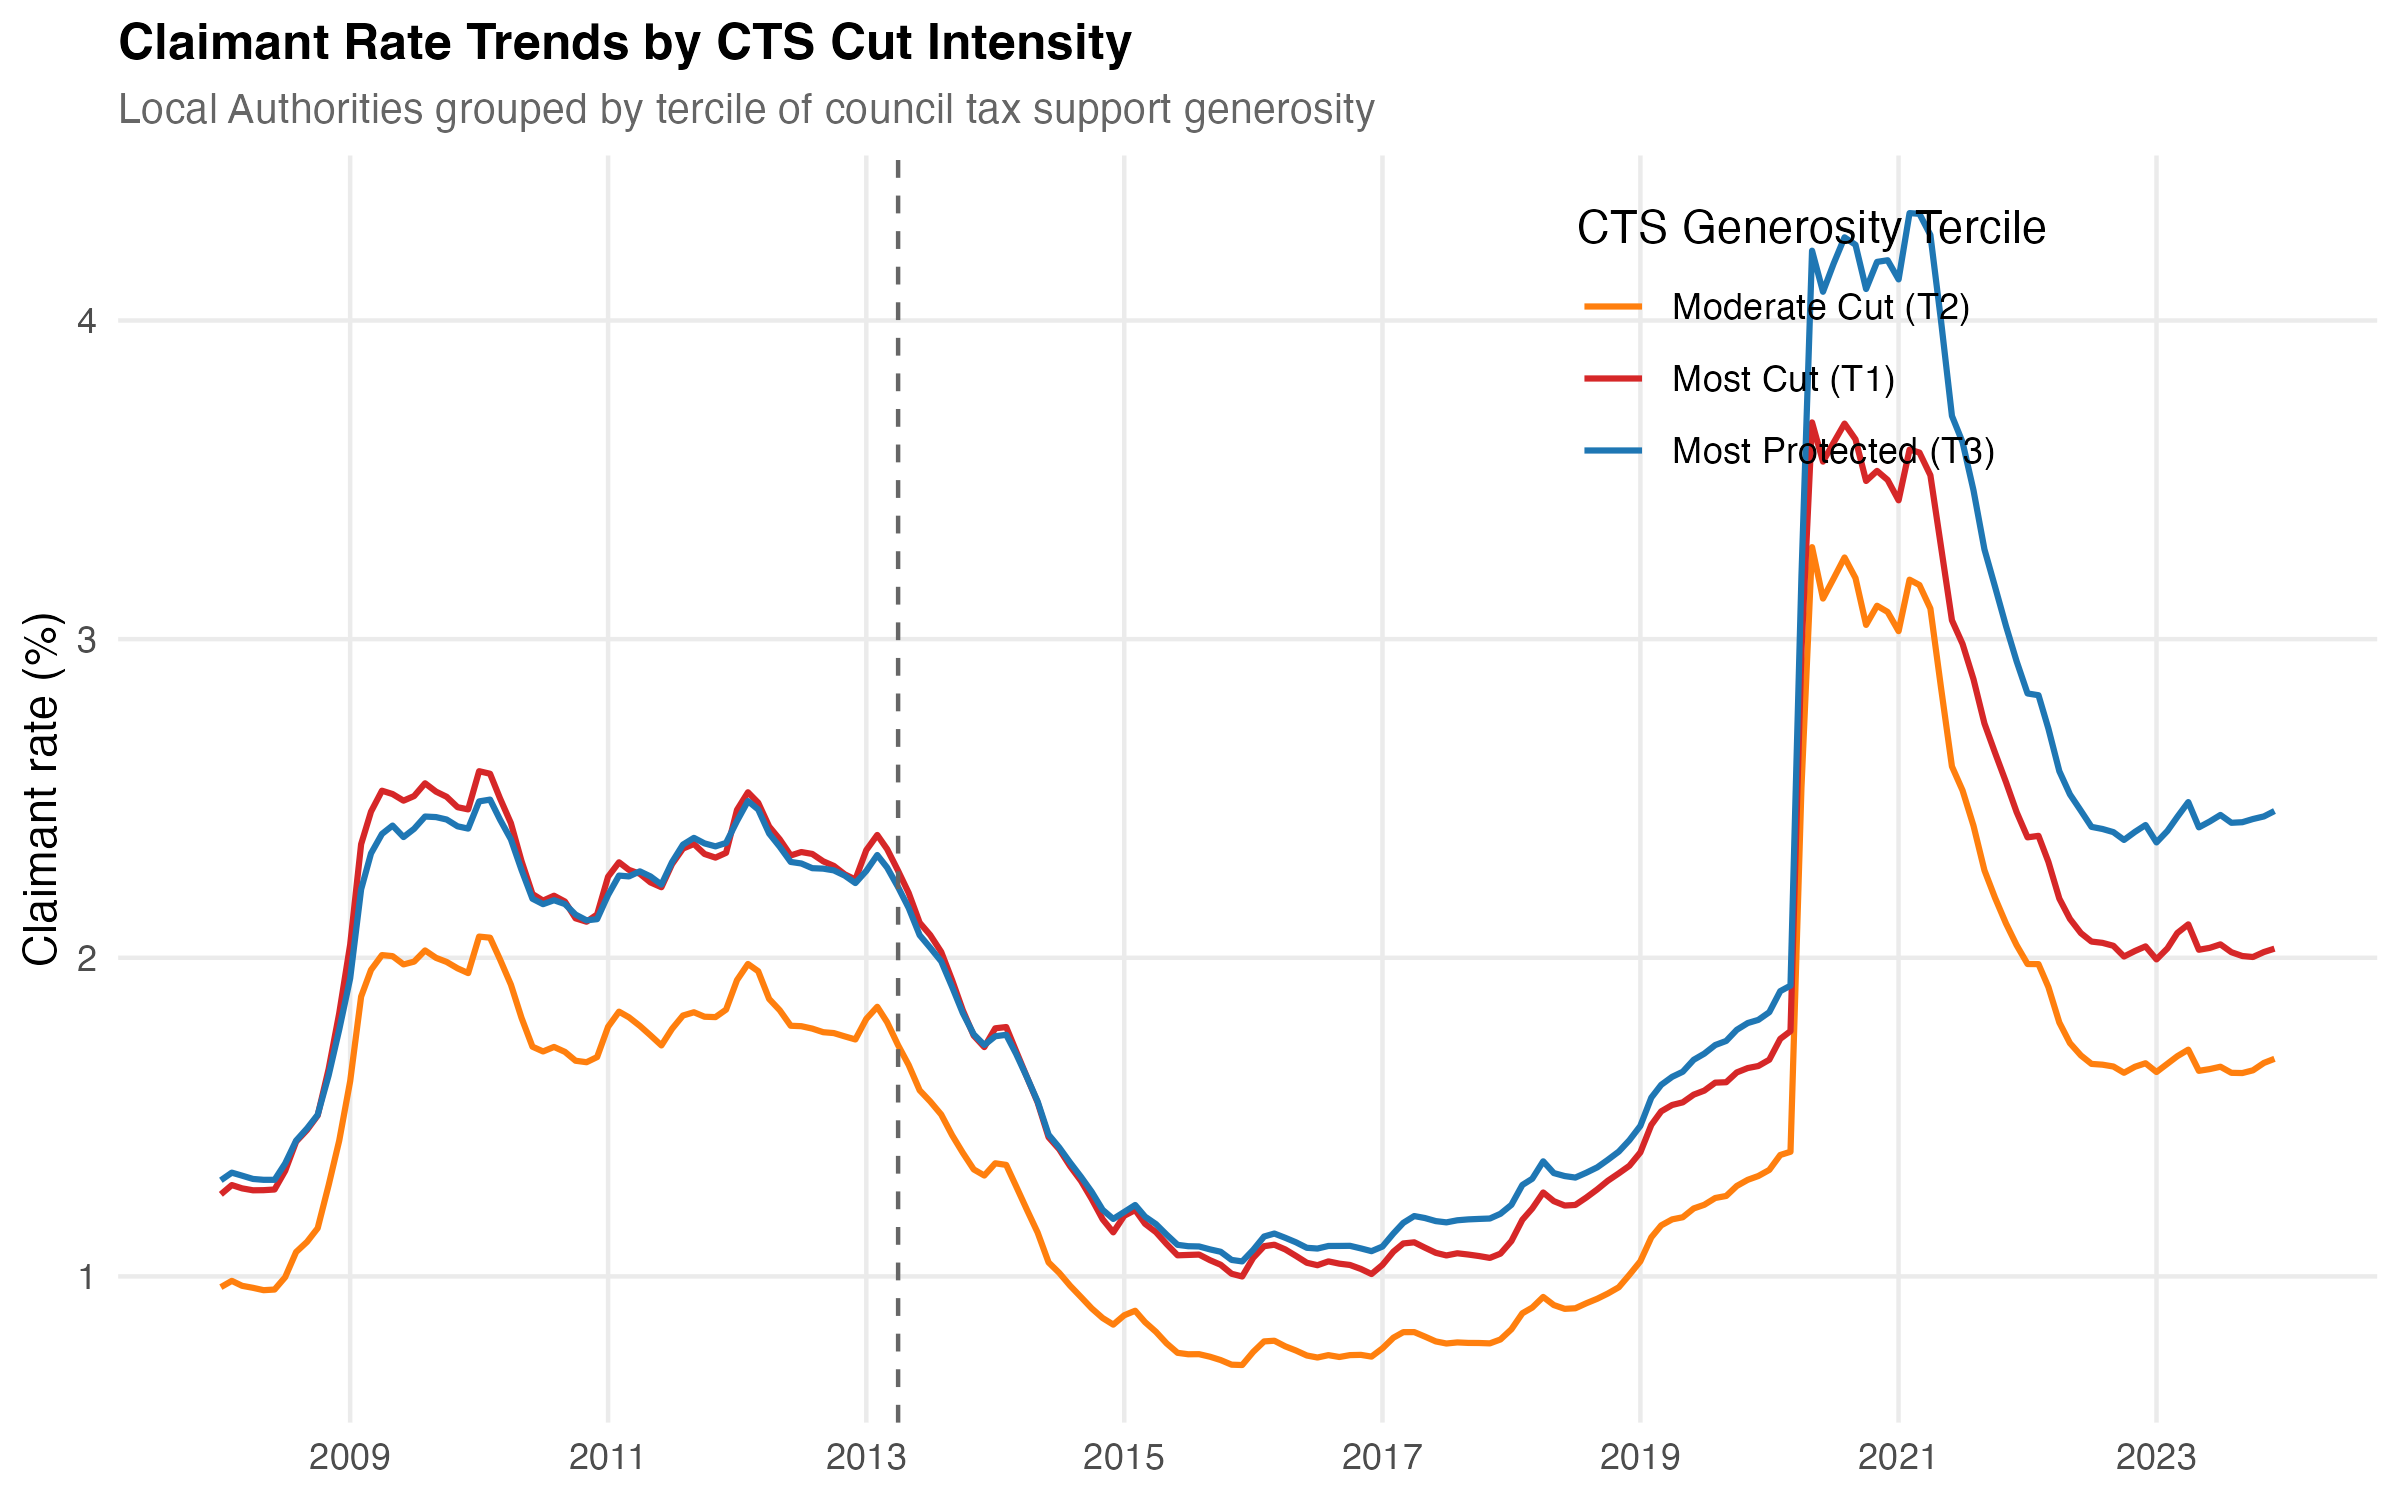
\includegraphics[width=0.9\textwidth]{figures/fig3_dose_response.png}
\caption{Claimant Rate Trends by CTS Cut Intensity (Terciles)}
\label{fig:dose_trends}
\floatfoot{\emph{Notes:} Monthly mean claimant rates by tercile of CTS generosity. T1 = most-cut authorities (lowest CTS per capita); T3 = most-protected. Dashed line marks April 2013. $N = 276$ local authorities.}
\end{figure}


\section{Discussion}

\subsection{Interpreting the Sign Reversal}

The central finding---that accounting for pre-trends reverses the estimated effect of CTS cuts from negative to positive---has two possible interpretations. Under the first, the detrended estimate is causal: CTS cuts genuinely increased claimant rates by approximately 0.15 percentage points, consistent with a financial distress channel. Under the second, the authority-specific trends over-correct, absorbing some of the true treatment effect along with the confounding trend.

I cannot definitively adjudicate between these interpretations. The pre-reform placebo is precisely null, suggesting that authority-specific linear trends do a good job of capturing the data-generating process in the pre-period. The HonestDiD analysis confirms that the naive estimate is fragile to even modest trend violations. However, the pre-2020 subsample analysis introduces an important caveat: when the COVID-19 period is excluded, both the naive and detrended estimates are statistically insignificant ($-$0.041 and $+$0.032, respectively). The sign pattern is preserved, but the magnitudes shrink substantially. This suggests that the full-sample significance is driven in part by differential COVID impacts on cut and protected authorities---a shock that occurred seven years after the reform and is unlikely to be causally downstream of CTS cuts alone.

The theoretical priors are mixed. While standard labour supply models predict that benefit cuts encourage work, the specific context---council tax for low-income households---involves amounts that are small relative to earnings but large relative to household budgets at the bottom of the distribution. The median minimum payment introduced by cut authorities was approximately \pounds 3--5 per week. At this level, the substitution effect (reduced implicit marginal tax rate) is trivially small, while the income effect (tighter household budget, risk of enforcement action for non-payment) may be substantial \citep{jrf2015council}.

A useful benchmark is the magnitude of the estimated effect. The trend-adjusted estimate of $+$0.152 percentage points implies that CTS cuts increased the claimant count by approximately 0.15 percent of the working-age population. Applied to the average cut authority (working-age population of 181,000), this translates to roughly 270 additional claimants per authority, or approximately 37,000 additional claimants nationwide across the 138 cut authorities. While not enormous in percentage terms, this is economically meaningful: it represents a welfare cost of the reform that partially offsets the fiscal savings from reduced CTS expenditure.

The magnitude is also consistent with back-of-envelope calculations from the financial distress channel. If the average minimum payment is \pounds 200 per year and roughly 5 percent of affected households experience sufficient financial distress to disrupt employment (e.g., through debt enforcement, loss of housing, or reduced job search intensity), the implied effect on authority-level claimant rates is on the order of 0.1--0.2 percentage points---precisely the range of the trend-adjusted estimate.

\subsection{Comparison with Prior Work}

My findings speak directly to two prior studies of CTS localisation. \citet{adam2019taxing} examined the labour supply effects of CTS reform using cross-sectional variation and found no significant employment effects. My panel design has several advantages: it tracks the same authorities over 16 years rather than comparing cross-sections, it includes explicit pre-trend diagnostics that reveal the confound in naive estimates, and it provides enough statistical power to detect effects of the magnitude found here. The null result in Adam et al.\ is consistent with my naive TWFE estimate (which, while significant, is confounded) if their cross-sectional approach also failed to account for pre-existing differences between cut and protected authorities.

\citet{fetzer2019austerity} used CTS cuts (among other austerity measures) to explain political outcomes, specifically support for Brexit. My finding that CTS cuts worsened labour market outcomes is consistent with Fetzer's political economy results: if CTS cuts increased financial distress and unemployment, the resulting economic grievance could plausibly manifest as anti-establishment political sentiment. The employment effects documented here provide a potential mechanism for the political effects documented by Fetzer.

More broadly, the results contribute to a growing scepticism about the employment effects of UK welfare reform. \citet{brewer2019did} found modest employment effects of the benefit cap, with the strongest responses concentrated among households closest to the cap threshold. The CTS context differs because the amounts involved are much smaller, the population is broader (all working-age claimants rather than just large families), and the policy operates through the council tax system rather than the benefit system directly. The common finding across these studies is that the employment response to benefit cuts among low-income UK households is either negligible or negative---far from the strong positive response predicted by simple incentive models.

\subsection{Mechanisms}

Why might CTS cuts worsen employment outcomes? I propose three channels, each grounded in evidence from the wider literature on poverty, financial distress, and labour market behaviour.

\emph{Financial distress and cognitive load.} Low-income households that suddenly owe council tax face a new, non-dischargeable obligation. Non-payment triggers summons costs (\pounds 80--120), liability orders, and ultimately bailiff enforcement. These financial pressures may divert time and cognitive resources from job search, consistent with the growing literature on scarcity and poverty traps \citep{chetty2013using}. The council tax enforcement process is particularly punitive: local authorities can apply for deductions directly from benefits, and the threat of bailiff action creates chronic stress that undermines the sustained, strategic job search behaviour needed to exit unemployment.

\emph{Debt spirals and housing instability.} Council tax arrears interact with other debts---rent arrears, fuel poverty, consumer credit---to create cascading financial difficulties that undermine housing stability and employment retention. The Joseph Rowntree Foundation documented sharp increases in council tax arrears following localisation, particularly in the least generous authorities \citep{jrf2015council}. In the most extreme cases, council tax debt can lead to imprisonment (committal for wilful refusal to pay), though this is rare. More commonly, the accumulation of multiple debts erodes the household's capacity to maintain the stability---reliable transport, appropriate clothing, internet access---that employment requires.

\emph{Administrative burden and take-up failure.} The transition from a national to local scheme created confusion and administrative errors. Some households lost support not because of policy design but because of failed transitions between benefit systems---a problem compounded by the simultaneous rollout of Universal Credit. Households that had previously received CTB automatically (it was administered alongside Housing Benefit) now needed to apply separately for local CTS, navigate unfamiliar application processes, and understand new eligibility rules that varied by authority. Administrative burden is increasingly recognised as a significant barrier to benefit take-up and labour market engagement \citep{chetty2013using}.

The relative importance of these channels cannot be disentangled with authority-level data alone. Individual-level administrative data linking council tax records, benefit receipt histories, and employment outcomes would allow researchers to decompose the aggregate effect into its constituent mechanisms. Such data exist within the DWP--HMRC administrative data infrastructure and the ADR UK Trusted Research Environment, though access requires specific research approvals.

\subsection{Policy Implications}

The findings have direct implications for the ongoing debate over welfare localisation in the UK. The government's stated rationale for CTS localisation was to give authorities ``a stake'' in getting residents into work---the idea that locally designed schemes would be more responsive to local conditions and more effective at encouraging employment than a one-size-fits-all national programme. My results suggest this reasoning was flawed: the authorities that exercised their discretion to cut support most aggressively did not see better employment outcomes. If anything, they saw worse ones.

This does not imply that localisation per se is harmful. It implies that localisation combined with a fiscal incentive to cut benefits (the 10 percent grant reduction) produced outcomes inconsistent with the reform's stated objectives. A localisation reform that maintained the overall funding envelope but allowed authorities to redesign CTS parameters (tapers, disregards, passporting thresholds) might have produced different results. The key distinction is between ``localisation as experimentation'' (authorities try different approaches with adequate resources) and ``localisation as austerity'' (authorities are forced to cut because the grant is insufficient).

The results also speak to the broader question of whether benefit cuts improve employment outcomes for low-income households. The standard economic model predicts positive effects through the substitution channel. But this model assumes that the margin of adjustment is labour supply, that job search is unconstrained, and that financial distress does not impair employment capacity. For households at the very bottom of the income distribution---those claiming council tax support---these assumptions may not hold. The amounts involved in CTS cuts (\pounds 3--5 per week) are too small to meaningfully change the return to work but large enough to trigger enforcement action and financial cascading that undermines employment.

\subsection{External Validity}

The findings are most directly relevant to the English context, where CTS localisation operates within a specific institutional framework (council tax, local authority administration, national benefit system). However, the broader lesson---that benefit cuts for low-income households may worsen rather than improve employment outcomes---has wider applicability. Similar dynamics have been documented in the US context, where aggressive welfare reform has sometimes pushed vulnerable households into deeper poverty without the predicted employment gains \citep{blank2002evaluating}.

The key mediating factor is likely the size of the benefit cut relative to household resources. For households with adequate savings, benefit cuts create genuine work incentives. For households already at subsistence, the same cuts trigger financial distress that overwhelms any substitution effect. The CTS context is informative precisely because the cuts were small enough to have minimal substitution effects but large enough to trigger enforcement cascading for households with no financial buffer.

\subsection{Limitations}

Several limitations warrant discussion. First, the claimant count is an imperfect measure of employment. It captures benefit receipt rather than actual employment status, and its definition changed substantially with the Universal Credit rollout. Under Jobseeker's Allowance, the claimant count captured a narrower population; under UC, it expanded to include all individuals in the ``searching for work'' conditionality group. The UC rollout was geographically staggered across job centres from 2013 to 2018, creating a potential confounder if rollout timing correlates with CTS generosity. While month fixed effects absorb national-level definitional changes and authority-specific trends absorb smooth differential rollout effects, the UC rollout is a first-order threat to identification that cannot be fully addressed without direct controls for UC rollout timing at the authority-month level---data that are not publicly available at the required granularity. This concern is particularly acute for the post-2018 period when UC was fully rolled out, and especially for the COVID period when UC claims surged nationwide.

Second, the treatment variable is measured at the authority level and captures average generosity rather than individual-level exposure. This ecological design may mask heterogeneity in the individual-level response to CTS cuts.

Third, the authority-specific linear trend specification imposes a parametric assumption on the form of the confounding trend. If the true confound is nonlinear, the trend-adjusted estimate may still be biased. The event-study evidence---showing that detrended pre-reform coefficients cluster around zero---provides some reassurance, but cannot rule out all forms of misspecification.

Fourth, I cannot directly observe the mechanism through which CTS cuts affect employment. Future work with individual-level administrative data linking council tax records to benefit receipt and employment histories would allow a more definitive test of the financial distress channel.



\section{Conclusion}

The 2013 localisation of Council Tax Support created the most significant cross-authority experiment in welfare generosity in recent English history. Exploiting this variation, I find that naive difference-in-differences estimates suggest CTS cuts improved employment outcomes---a finding that aligns with standard work incentive theory and would support further welfare retrenchment.

But this headline result is unreliable. Event-study diagnostics reveal significant pre-trends: cut authorities were already on steeper downward claimant trajectories before the reform. Controlling for these trends reverses the estimated effect: the trend-adjusted estimate suggests that CTS cuts \emph{increased} claimant rates by 0.15 percentage points, consistent with financial distress dominating work incentive effects. However, restricting to the pre-COVID period renders both estimates statistically insignificant, suggesting that the full-sample significance partly reflects differential pandemic impacts rather than the reform alone.

The methodological lesson is as important as the substantive one. Standard two-way fixed effects can produce confident, significant, and wrong estimates when treatment groups differ in their pre-existing trajectories. The sign reversal documented here is not a curiosity but a warning: without careful pre-trend diagnostics, quasi-experimental estimates can tell exactly the story that policymakers want to hear, regardless of the underlying truth.

For policy, the findings suggest caution about further localisation of means-tested benefits. The CTS reform was motivated by a desire to give local authorities ``skin in the game'' and to reduce the welfare bill. But the employment costs of benefit cuts---mediated through financial distress, debt, and administrative burden---may offset or exceed the fiscal savings. At a minimum, the null-to-positive effect on claimant rates suggests that CTS cuts did not produce the employment gains that their proponents anticipated.

The methodological lesson deserves equal emphasis. Pre-trend diagnostics are not optional robustness checks---they are essential for the credibility of any difference-in-differences design. In this case, the sign reversal between naive and trend-adjusted estimates changes the policy conclusion from ``CTS cuts reduced unemployment'' to ``CTS cuts may have increased unemployment.'' Without the event study and the HonestDiD analysis, the naive estimate would pass standard significance tests and tell a coherent theoretical story. Only careful scrutiny of the identifying assumptions reveals that this story is driven by confounding rather than causation. As applied researchers increasingly rely on quasi-experimental designs for policy evaluation, the CTS case serves as a cautionary tale about the consequences of taking parallel trends on faith.

Several avenues for future research emerge from this analysis. First, individual-level administrative data from the DWP--HMRC Longitudinal Education Outcomes dataset or the ADR UK Trusted Research Environment could provide direct evidence on the mechanisms connecting CTS cuts to employment outcomes, including the role of council tax arrears, enforcement action, and housing instability. Second, the long post-reform period (2013--2023) allows researchers to examine whether the effects of CTS cuts evolved over time---whether authorities and households adapted, or whether the initial shock had persistent effects. Third, the interaction between CTS localisation and subsequent welfare reforms (particularly Universal Credit rollout) deserves attention: did UC mitigate or amplify the effects of CTS cuts by changing the overall benefit landscape?

Finally, the CTS experience has direct relevance for current policy debates. The UK government continues to devolve welfare responsibilities to local authorities, and the tension between fiscal consolidation and social protection remains central to public policy. Understanding whether---and under what conditions---benefit localisation improves or harms employment outcomes is critical for designing welfare systems that achieve their stated objectives without imposing unintended costs on the most vulnerable households.


\section*{Acknowledgements}

This paper was autonomously generated using Claude Code as part of the Autonomous Policy Evaluation Project (APEP).

\noindent\textbf{Project Repository:} \url{https://github.com/SocialCatalystLab/ape-papers}

\noindent\textbf{Contributors:} @olafdrw

\noindent\textbf{First Contributor:} \url{https://github.com/olafdrw}

\label{apep_main_text_end}
\newpage
\bibliography{references}


\newpage
\appendix

\section{Data Appendix}
\label{app:data}

\subsection{Data Sources}

\begin{enumerate}
\item \textbf{Claimant Count.} NOMIS dataset NM\_162\_1, ``Claimant count -- monthly local authority district.'' Downloaded via the NOMIS API (\url{https://www.nomisweb.co.uk/api/v01/}). Coverage: January 2008 to December 2023. Geographic level: local authority district (2023 boundaries). Measure: all persons claiming unemployment-related benefits (Jobseeker's Allowance or Universal Credit ``searching for work'' conditionality group). The raw extract contains 77,952 observations across 406 authority codes (including Scotland and Wales); after restricting to English authorities (GSS codes starting with ``E''), 62,592 observations across 326 authorities remain.

\item \textbf{Council Taxbase (LCTS 2013).} DLUHC ``Council Taxbase'' series, 2013 edition. Downloaded from GOV.UK.\footnote{\url{https://www.gov.uk/government/statistics/council-taxbase-2013-in-england}} The ``Data'' sheet records council tax support cases by valuation band, separately for pensioners (columns 4--13), working-age claimants (columns 14--23), and all claimants (columns 24--33). Band totals are in columns 13, 23, and 33 respectively. I use the working-age total (column 23) and grand total (column 33) for each billing authority.

\item \textbf{Population Estimates.} ONS mid-year population estimates by local authority, accessed via NOMIS. Age group: 16--64 (working age). Coverage: 2008--2023. Used to construct the claimant rate denominator and to normalise CTS expenditure per capita.
\end{enumerate}

\subsection{Treatment Variable Construction}

The treatment variable is constructed in four steps:

\begin{enumerate}
\item \textbf{CTS per capita:} $\text{CTS}_{a}^{\text{pc}} = \text{Working-age CTS}_{a} / \text{Pop}_{a}^{16\text{--}64}(2012)$

\item \textbf{Residualisation:} Regress $\text{CTS}_{a}^{\text{pc}}$ on the pre-reform mean claimant rate (2010--2012). The residual captures generosity beyond what baseline labour market conditions would predict. The $R^2$ of this regression is 0.455, indicating that about half of the cross-authority variation in CTS per capita is explained by pre-reform claimant rates.

\item \textbf{Binary treatment:} Authorities with below-median residual are classified as ``cut'' ($N = 138$); above-median as ``protected'' ($N = 138$).

\item \textbf{Continuous treatment:} The standardised residual (mean 0, SD 1) provides continuous treatment intensity. Tercile groups split authorities into most-cut (T1), moderate (T2), and most-protected (T3).
\end{enumerate}

\subsection{Sample Restrictions}

Starting from 326 English local authorities in NOMIS:
\begin{itemize}
\item $-$42: Failed name-matching between NOMIS (ONS GSS codes) and DLUHC (billing authority codes)
\item $-$8: Missing population data or zero working-age population
\item Final sample: 276 authorities $\times$ 192 months $=$ 52,992 observations
\end{itemize}

The unmatched authorities are primarily small district councils with name changes or mergers between 2012 and 2023. The matched sample covers 85\% of English authorities and 91\% of the English working-age population.


\section{Identification Appendix}
\label{app:identification}

\subsection{Pre-Trend Diagnostics}

\Cref{tab:pretrends} reports the pre-reform event-study coefficients from the raw TWFE specification. The joint Wald test for pre-reform coefficients being zero is rejected at all conventional significance levels, confirming the failure of parallel trends in the naive specification.

\begin{table}[H]
\centering
\caption{Pre-Reform Event Study Coefficients (Raw TWFE)}
\label{tab:pretrends}
\begin{threeparttable}
\begin{tabular}{ccc}
\toprule
Quarter & Estimate & Std. Error \\
\midrule
$-$8 & $-$0.0231 & 0.0347 \\
$-$7 & $-$0.0563** & 0.0236 \\
$-$6 & $-$0.0664*** & 0.0192 \\
$-$5 & $-$0.0263* & 0.0135 \\
$-$4 & $-$0.0343** & 0.0139 \\
$-$3 & $-$0.0240* & 0.0141 \\
$-$2 & $-$0.0362*** & 0.0092 \\
\bottomrule
\end{tabular}
\begin{tablenotes}[flushleft]
\small
\item \emph{Notes:} Coefficients from the event-study specification (Equation~\ref{eq:eventstudy}), pre-reform periods only. Reference period: $q = -1$. * $p<0.10$, ** $p<0.05$, *** $p<0.01$.
\end{tablenotes}
\end{threeparttable}
\end{table}

The monotonic increase in the absolute magnitude of pre-reform coefficients as we move further from the reform date is consistent with a smooth linear divergence---exactly the pattern that authority-specific linear trends are designed to capture. If the pre-trend were driven by anticipation (e.g., cut authorities adjusting before the reform), we would expect coefficients to increase in magnitude only in the 2--3 quarters immediately preceding the reform, not 6--8 quarters prior.

\subsection{HonestDiD Sensitivity}

I apply the \citet{rambachan2023more} sensitivity framework to assess how robust the main TWFE estimate is to departures from parallel trends. The parameter $M$ bounds the maximum change in the slope of the parallel trends violation between consecutive periods. At $M = 0$ (strict parallel trends), the identified set for the treatment effect is $\{-0.156\}$. At $M = 0.01$---allowing the parallel trends violation to increase by 0.01 percentage points per quarter---the identified set widens to include zero. At $M = 0.03$, the identified set shifts entirely to positive values, consistent with the trend-adjusted point estimate of $+$0.152.


\section{Robustness Appendix}
\label{app:robustness}

\subsection{Leave-One-Out Analysis}

Dropping each of the ten largest local authorities (by working-age population) produces baseline TWFE estimates ranging from $-$0.168 to $-$0.161 percentage points, all highly significant. The narrow range confirms that the naive result is not driven by any single large authority.

\subsection{Treatment Distribution}

\Cref{fig:treatment_dist} shows the distribution of working-age CTS per capita across authorities. The distribution is right-skewed, with a median of \pounds 33.18 and a mean of \pounds 36.12. The dashed line marks the median used for binary treatment classification.

\begin{figure}[H]
\centering
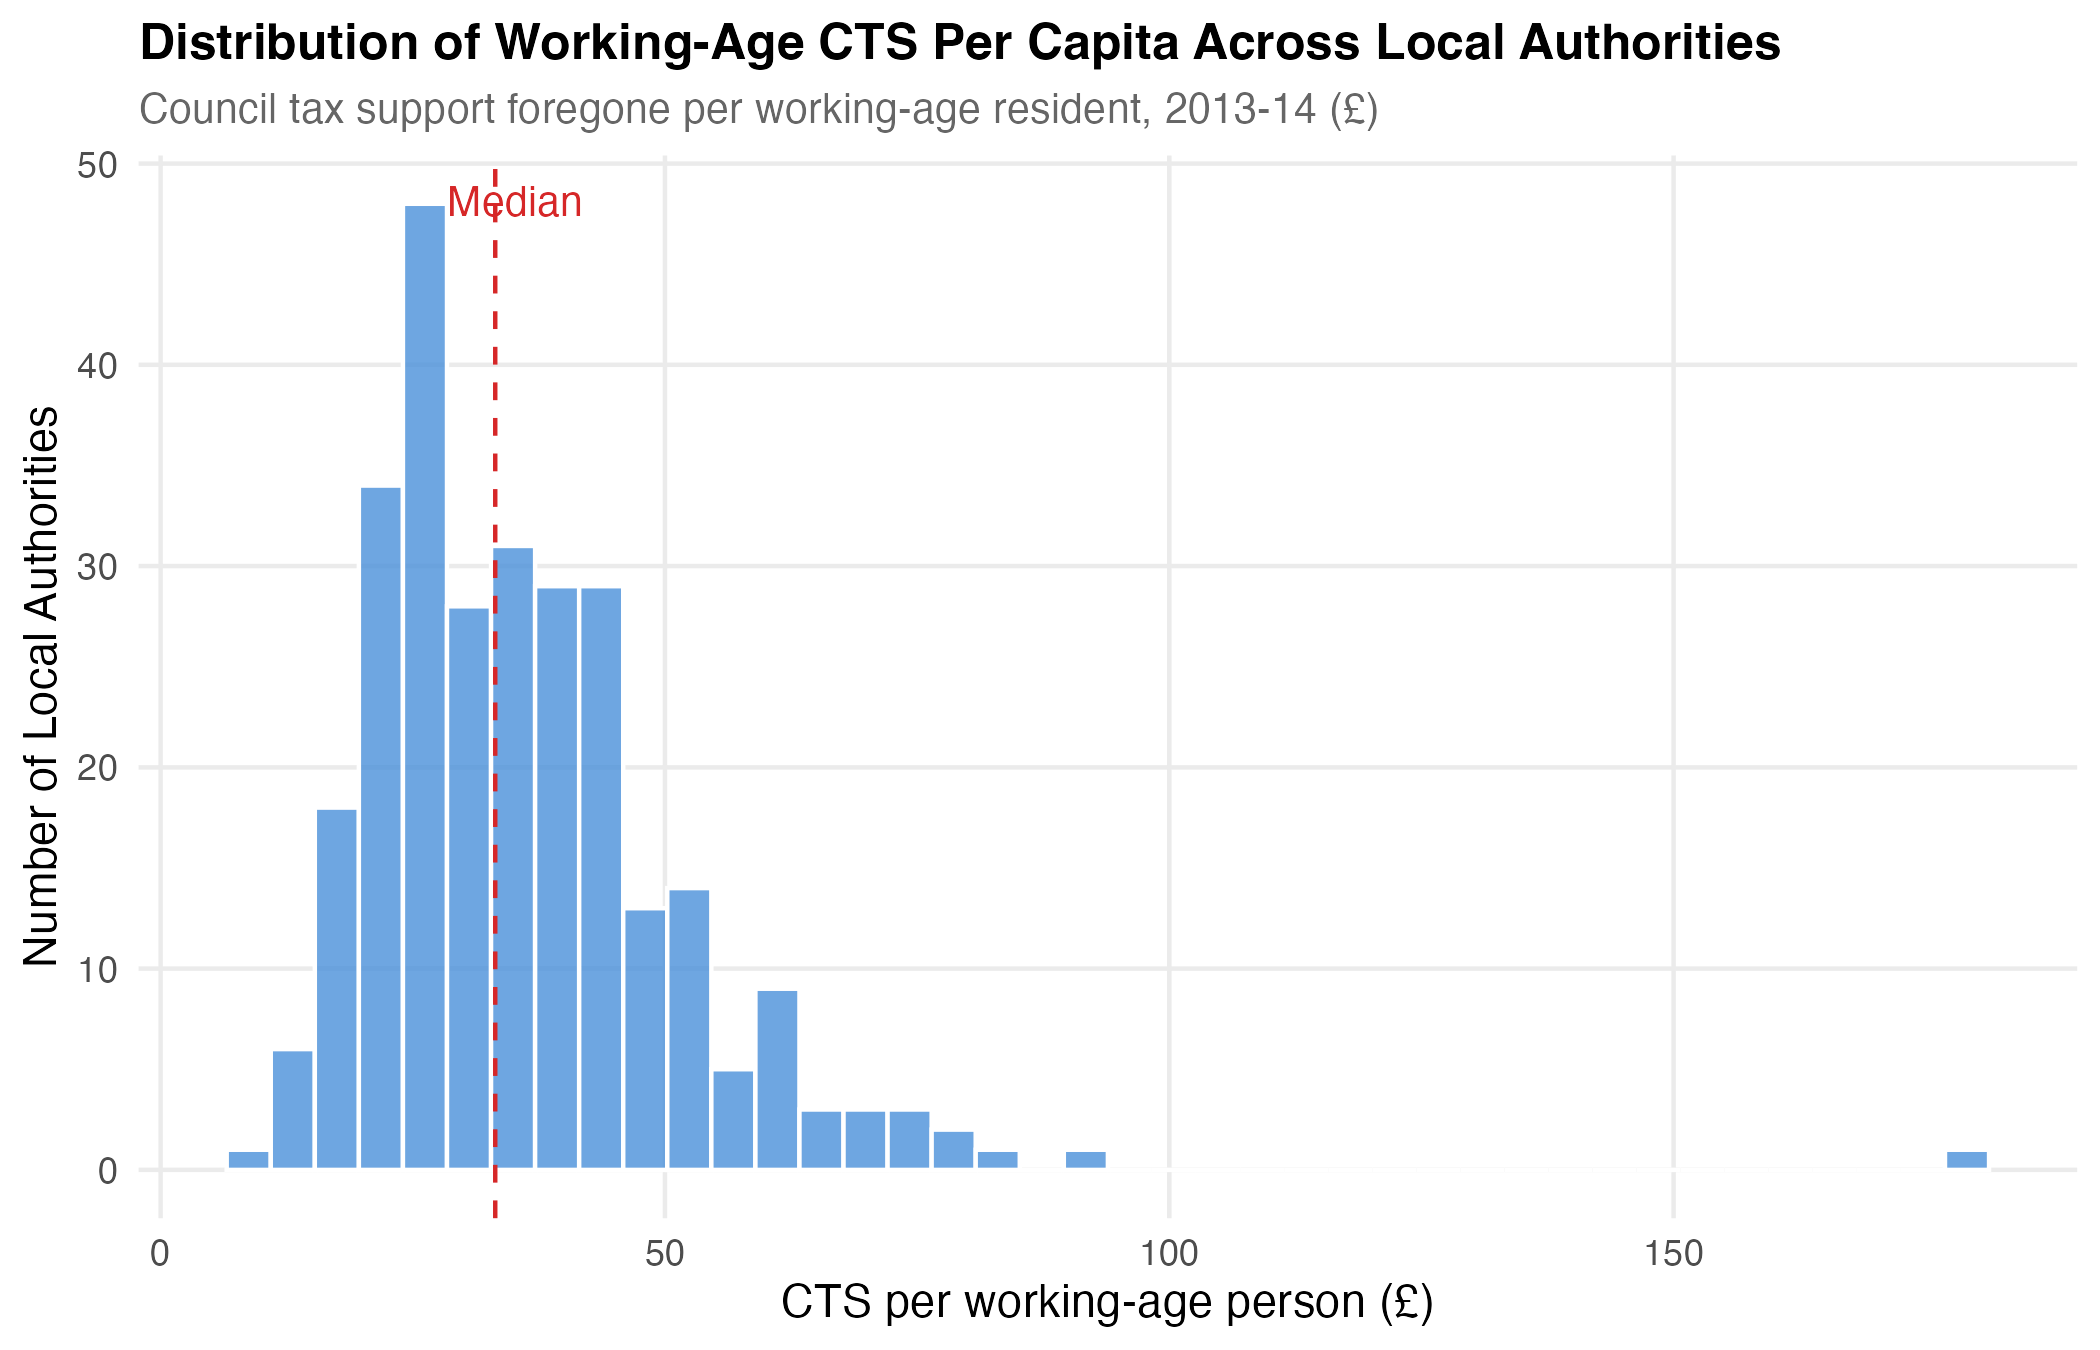
\includegraphics[width=0.85\textwidth]{figures/fig4_treatment_dist.png}
\caption{Distribution of Working-Age CTS Per Capita}
\label{fig:treatment_dist}
\floatfoot{\emph{Notes:} Histogram of working-age Council Tax Support expenditure per working-age person (2012 population) across English local authorities. Based on DLUHC Council Taxbase 2013 data. Dashed line indicates the median (\pounds 33.18). $N = 276$ matched authorities.}
\end{figure}


\section{Additional Tables and Figures}
\label{app:additional}

All figures and tables are available in the replication archive. The R code that generates all exhibits is provided in the \texttt{code/} directory of the replication package:
\begin{itemize}
\item \texttt{00\_packages.R}: Package loading and setup
\item \texttt{01\_fetch\_data.R}: Data acquisition from NOMIS and DLUHC
\item \texttt{02\_clean\_data.R}: Panel construction and treatment variable
\item \texttt{03\_main\_analysis.R}: Primary DiD estimation and event study
\item \texttt{04\_robustness.R}: Robustness checks and sensitivity analysis
\item \texttt{05\_figures.R}: All figures
\item \texttt{06\_tables.R}: All tables
\end{itemize}

\end{document}
